\documentclass[11pt]{beamer}

\usetheme{Madrid}
\usecolortheme{whale}

\usepackage[utf8]{inputenc}
\usepackage[T1]{fontenc}
\usepackage{amsmath,amssymb}
\usepackage{graphicx}
\usepackage{hyperref}
\usepackage{tikz}
\usepackage{booktabs}

\title[Neural Operator Tutorial]{A Practical Introduction to\\Neural Operators for PDEs}
\subtitle{Solving Partial Differential Equations with Deep Learning}
\author[Smith \& Chen]{John Smith \and Maria Chen}
\institute{University of Technology}
\date{ICML Workshop, July 2026}

\begin{document}

\begin{frame}
    \titlepage
\end{frame}

\begin{frame}{Outline}
    \tableofcontents
\end{frame}

\section{Motivation}

\begin{frame}{Why Learn PDE Solvers?}
    \begin{block}{The Challenge}
        Traditional PDE solvers (FEM, FDM, FVM) are:
        \begin{itemize}
            \item Computationally expensive for fine discretizations
            \item Require re-solving for each new set of parameters
            \item Poor at leveraging data from similar problems
        \end{itemize}
    \end{block}

    \pause

    \begin{alertblock}{The Opportunity}
        Neural operators learn the \emph{mapping between function spaces}, enabling:
        \begin{itemize}
            \item Zero-shot generalization to new discretizations
            \item Amortized inference: train once, evaluate many times
            \item Data-driven discovery from observations
        \end{itemize}
    \end{alertblock}
\end{frame}

\section{Mathematical Formulation}

\begin{frame}{Problem Setup}
    We want to solve parametric PDEs of the form:

    \begin{equation}
        \mathcal{L}_a[u](x) = f(x), \quad x \in D \subset \mathbb{R}^d
        \label{eq:pde}
    \end{equation}

    \pause

    \begin{block}{Goal}
        Learn an operator $\mathcal{G}_\theta : \mathcal{A} \rightarrow \mathcal{U}$ that maps
        \begin{itemize}
            \item Input function $a \in \mathcal{A}$ (coefficients, forcing, BCs)
            \item To solution $u \in \mathcal{U}$
        \end{itemize}
        such that $\mathcal{G}_\theta(a) \approx u$.
    \end{block}
\end{frame}

\begin{frame}{Fourier Neural Operator (FNO)}
    \begin{columns}
        \column{0.45\textwidth}
        The FNO architecture \cite{li2020fourier}:
        \begin{enumerate}
            \item Lift: $v_0(x) = P(a(x))$
            \item Fourier layers:
            \begin{equation*}
                v_{t+1}(x) = \sigma\left(
                    W v_t(x) + \mathcal{F}^{-1}(R \cdot \mathcal{F}[v_t])(x)
                \right)
            \end{equation*}
            \item Project: $u(x) = Q(v_T(x))$
        \end{enumerate}

        \column{0.5\textwidth}
        \centering
        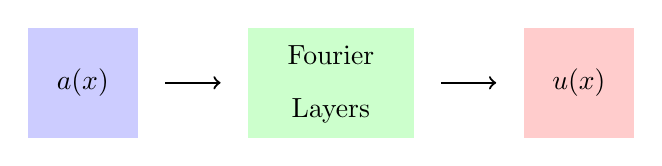
\begin{tikzpicture}[scale=0.7]
            \fill[blue!20] (0,0) rectangle (2,2);
            \node at (1,1) {$a(x)$};
            \draw[->, thick] (2.5,1) -- (3.5,1);
            \fill[green!20] (4,0) rectangle (7,2);
            \node at (5.5,1.5) {Fourier};
            \node at (5.5,0.5) {Layers};
            \draw[->, thick] (7.5,1) -- (8.5,1);
            \fill[red!20] (9,0) rectangle (11,2);
            \node at (10,1) {$u(x)$};
        \end{tikzpicture}
    \end{columns}
\end{frame}

\begin{frame}{Key Properties of Neural Operators}
    \begin{theorem}[Universal Approximation]
        Neural operators can approximate any continuous operator to arbitrary accuracy
        \cite{kovachki2023neural}.
    \end{theorem}

    \pause

    \begin{block}{Discretization Invariance}
        \begin{itemize}
            \item Trained on one grid resolution
            \item Evaluates correctly on \emph{any} resolution
            \item Key advantage over classical CNNs
        \end{itemize}
    \end{block}
\end{frame}

\section{Applications}

\begin{frame}{Benchmark: Darcy Flow}
    \begin{equation}
        -\nabla \cdot (a(x) \nabla u(x)) = f(x), \quad x \in [0,1]^2
    \end{equation}

    \begin{table}
        \centering
        \caption{Relative $L^2$ error on Darcy flow}
        \begin{tabular}{@{}lcc@{}}
            \toprule
            Method    & $64\times64$ & $128\times128$ \\
            \midrule
            FNO-2D    & 0.0082 & 0.0089 \\
            U-Net     & 0.0245 & 0.0312 \\
            DeepONet  & 0.0123 & 0.0141 \\
            \bottomrule
        \end{tabular}
    \end{table}
\end{frame}

\section{Conclusion}

\begin{frame}{Takeaways}
    \begin{itemize}
        \item Neural operators learn mappings between \emph{infinite-dimensional} function spaces
        \item Discretization invariance enables flexible deployment
        \item State-of-the-art for parametric PDE families
        \item Active area: combining with physics-informed losses
    \end{itemize}

    \vspace{1cm}

    \begin{center}
        \Large{\textbf{Thank you!}}\\
        \vspace{0.3cm}
        \small{Code: \url{github.com/neural-operators}}\\
        \small{Contact: \texttt{jane@neural-operator.org}}
    \end{center}
\end{frame}

\begin{frame}[allowframebreaks]{References}
    \bibliographystyle{plain}
    \begin{thebibliography}{9}

    \bibitem{li2020fourier}
    Z.~Li et al.
    \newblock Fourier neural operator for parametric PDEs.
    \newblock In \emph{ICLR}, 2021.

    \bibitem{kovachki2023neural}
    N.~Kovachki et al.
    \newblock Neural operator: Learning maps between function spaces.
    \newblock In \emph{JMLR}, 2023.

    \end{thebibliography}
\end{frame}

\end{document}
